%! Author = vsharma
%! Date = 25.09.2022
% !TeX spellcheck = en_EN

\chapter{Evaluation}

\par In this chapter, based on the approaches from the
previous chapter, the efficiency of
Prowler is evaluated against security vulnerabilities.
The result of the evaluation of each approach is discussed here.

\par In the end, a comparison between the assessment of security vulnerabilities performed using Prowler and
ScoutSuite is also highlighted which showcases the efficiency of each tool individually.

\section{Using Test Driven Approach}
\begin{figure}
    \centering
    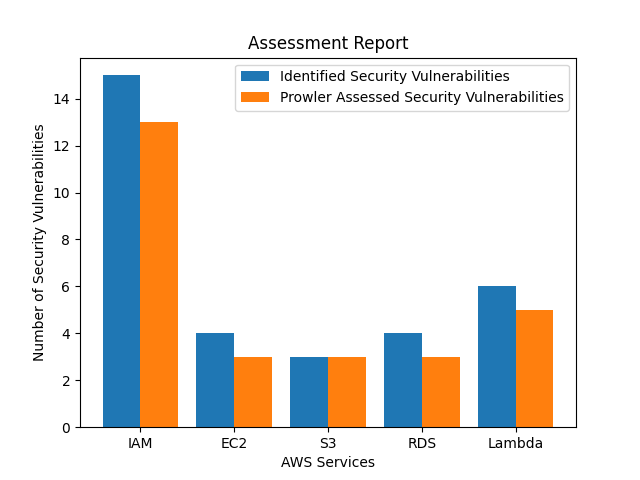
\includegraphics[width=\textwidth]{assessmentgraph.png}
    \caption{Prowler Assessment Graph}
    \label{fig:prowlerefficiency}
\end{figure}

\par The test-driven approach requires developing the test cases for the possible assessable scenario of a check in Prowler that performs the security assessment of an identified security vulnerability in the AWS service.
The individual test cases are developed, and their results are noted.

\par The checks in Prowler corresponding to the identified security vulnerabilities are identified manually.
The functionality of the check is understood and verified if the check can perform the assessment of the identified security vulnerability.
The verification process includes developing test cases for all assessable scenarios and evaluating the result of the assessment.
Only if all the scenarios are successfully verified the security vulnerability is marked to be assessed using Prowler.
Once all the test scenarios for the different checks in Prowler are developed and verified, the efficiency of Prowler is calculated against the identified security vulnerabilities for individual AWS services.
The efficiency calculation is done programmatically.

\begin{longtable}{|p{10cm}|p{2.4cm}|p{2cm}|}
    \hline
    \textbf{Security Vulnerabilities} & \textbf{Service} & \textbf{Prowler Check}\\
    \hline
    Avoid the use of the root account & IAM & Check11 \\
    \hline
    MFA is enabled for all IAM users & IAM & Check12 \\
    \hline
    Credentials unused for 90 days or greater are disabled & IAM & Check13 \\
    \hline
    Access keys are rotated every 90 days or less & IAM & Check14 \\
    \hline
    IAM password policy requires at least one uppercase letter & IAM & Check15 \\
    \hline
    IAM password policy requires at least one lowercase letter & IAM & Check16 \\
    \hline
    IAM password policy requires at least one symbol & IAM & Check17\\
    \hline
    IAM password policy requires at least one number & IAM & Check18\\
    \hline
    IAM password policy requires a minimum length of 14 or greater & IAM & Check19\\
    \hline
    IAM password policy prevents password reuse & IAM & Check110\\
    \hline
    IAM password policy expires passwords within 90 days or less & IAM & Check111\\
    \hline
    Password expiration requires an administrator reset & IAM & \\
    \hline
    Allow users to change their own password & IAM& \\
    \hline
    Insider Threat & IAM & Extra774\\
    \hline
    Access key for the root account & IAM & Check112 \\
    \hline
    Instances created from Malicious AMI & EC2 & Check76\\
    \hline
    User data public exposure & EC2 & Extra741\\
    \hline
    Server-Side Request Forgery & EC2 & Extra786\\
    \hline
    Denial of Wallet & EC2, Lambda &\\
    \hline
    Public exposure of S3 buckets & S3 & Check73\\
    \hline
    Unencrypted S3 buckets & S3 & Extra764\\
    \hline
    GhostWriter & S3 & Extra771 \\
    \hline
    Publicly accessible RDS instances & RDS & Check78\\
    \hline
    Unencrypted RDS Instance & RDS & Extra735\\
    \hline
    Resources running in an AWS classic resource & RDS & \\
    \hline
    Default data retention & RDS & Extra739\\
    \hline
    Lambda functions have a public resource-based policy & Lambda & Extra798 \\
    \hline
    Publicly accessible AWS account & Lambda & Extra7145 \\
    \hline
    Public lambda function URL & Lambda & Extra7179 \\
    \hline
    Public lambda function URL Cors & Lambda & Extra7180 \\
    \hline
    Insecure Management of Secrets & Lambda & Extra760\\
    \hline
    Poisoning the Well & Lambda & \\
    \hline
    \caption{Prowler Checks and mapped Security Vulnerabilities}
    \label{tab:securityvulnerabilitiescheckin prowler}
\end{longtable}

\par The process for calculating the efficiency of Prowler begins by determining the count of the security vulnerabilities that are identified for an AWS service.
The table \ref{tab:classificationofsecurityvulnerabilities} shows all the security vulnerabilities that are identified in the five AWS services.
Additionally, the table also highlights the different checks in Prowler that are identified and verified by developing the test cases that assess these identified security vulnerabilities.
The count of number of security vulnerabilities that are identified for the AWS service is determined.
Also, the number of security vulnerabilities that are assessed using Prowler for that AWS service is determined.
Based on these results the efficiency of Prowler is calculated in assessing an AWS service.
For example, looking at the table \ref{tab:classificationofsecurityvulnerabilities} and the graph \ref{fig:prowlerefficiency} considering AWS RDS, the number of identified security vulnerabilities is 4, and the number of security vulnerabilities that are assessed using Prowler is 3.
This process is performed for the 5 AWS services that are chosen for this research work.
In the end, it is possible to determine how efficient Prowler is in assessing the security vulnerabilities of each AWS service.


\par The graph \ref{fig:prowlerefficiency} is drawn between the AWS services considered for this thesis work and the number of security vulnerabilities.
It highlights the total number of security vulnerabilities identified for an AWS service and the number of security vulnerabilities that are assessed using Prowler for the AWS service.

\par Looking at the graph for IAM, it can be concluded that out of the 15 identified security vulnerabilities, Prowler performs the assessment of 13 security vulnerabilities.
The 2 security vulnerabilities that cannot be assessed by Prowler are \textit{Password expiration requires administrator reset} and \textit{Allow users to change their own password}.
These security vulnerabilities are caused due to excessive privilege.
The Password expiration requires an administrator reset feature prevents the user from updating their password after the account password has expired and thus requires administrative access.
This causes an issue on the user’s productivity and increases the workload on the administrator but ensures account safety.
If the account user is given administrative permission, this avoids the impact on the user’s productivity, but at the same time increases the risk that the user can cause.
This user can reset passwords for another user, revoke or grant unrestricted access to resources, files or directories and can even delete other user resources or accounts.
The allows users to change their own password feature enables all the users to change their own account password thus ensuring only the user of the account should be able to change the password for his account.
If the user is granted an administrative role, the user would not just be able to change the password for his own account but would be able to manage other user accounts as well.
Assigning excessive privilege to a user can lead to 
deadly sin such as siphoning important information to the
competitors, data destruction, etc \cite{87}.

\par Like IAM, looking at the graph for EC2 it can be determined that out of the 4 identified security vulnerabilities, 3 of those security vulnerabilities are assessed using Prowler.
 The unassessed security vulnerability using Prowler is the Denial of wallet.
 Most of the time data loss incidents make the news, but the denial of wallet is one of the common ways that can be found out about a compromise through the AWS bill.
 The denial of wallet security vulnerability causes 
disruption of the target system or flooding the system 
with traffic as a form of threat, ransom, or revenge thus
depriving the system usage or leading to downtime 
resulting in loss of time and money, and reputation \cite{86}.

\par Prowler shows 100 \% efficiency in assessing the security vulnerabilities that are identified in S3 and thus Prowler is highly efficient in performing the security best practices assessments, audits, and incident response for S3.

\par Similar to IAM and EC2, out of 4 identified security
vulnerabilities prowler performs the assessment of 3 security vulnerabilities.
Prowler does not perform the assessment of security vulnerability that can occur due to RDS instances running on AWS classic resources.
The EC2-Classic platform is retired by Amazon and disabled on all accounts.
The EC2-Classic platform is replaced the EC2-VPC \cite{88}.

\par As seen from the graph \ref{fig:prowlerefficiency}, out of the 6 security vulnerabilities identified in AWS lambda, Prowler can perform the assessment of 5 security vulnerabilities.
The security vulnerability that is not assessed using Prowler is ‘Poisoning of well’.
Poisoning of well can be highly hazardous in numerous ways.
It can occur when the malicious users inject fake
training
data with the aim of corrupting the learned model and can
spread, affecting the products that draw from it or when
an Integrated Development Environment (IDE) plugin hosting the cloud server is controlled by an attacker.
A code backdoor is introduced as the security vulnerability by the attacker into the plugin \cite{89}.


\section{Using Open-Source Application}

\begin{figure}
    \centering
    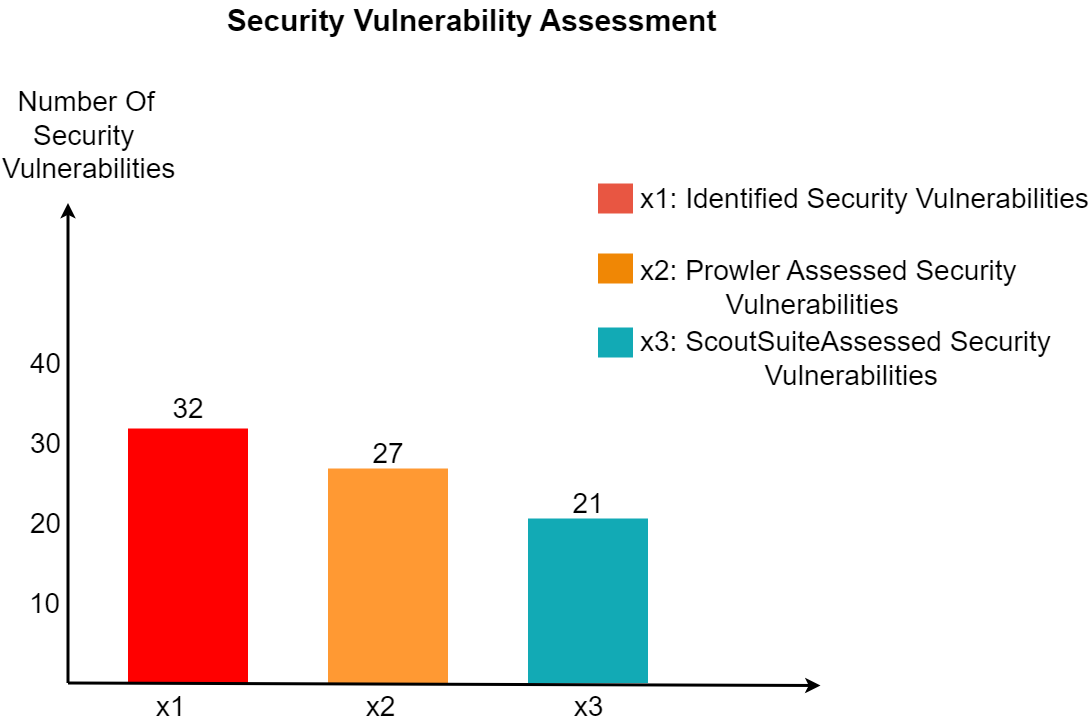
\includegraphics[width=\textwidth]{prowlervsscoutsuite.png}
    \caption{Security Vulnerabilities Assessment Graph}
    \label{fig:prowlervsscoutsuite}
\end{figure}

\par Cloud service providers make tools available to secure the cloud systems, but it is ultimately the user’s responsibility to use them.
The control needed to define and implement the cloud infrastructure differs greatly from the controls used in on-premises environments.
Simply transforming the hardware servers to AWS EC2 instances won't make the infrastructure secure by default.
This is because, while AWS is responsible for the
security of the cloud, it is the users responsibility
for the security in the cloud.
Due to this, many companies suffer from misconfigured and poorly architected cloud infrastructure, leading to embarrassing data leaks \cite{74}.
This section shows the assessment of security vulnerability performed using two open-source cloud security assessment tools namely Prowler and ScoutSuite which can help strengthen the cloud security posture without breaking the bank.

\par The employee management web application \cite{69} leverages different AWS services namely IAM, EC2, S3, RDS, and Lambda for its deployment on AWS cloud infrastructure as shown in the figure \ref{fig:infrastructure_architecture}.
Once the application is deployed on the AWS cloud, the application functionality is verified.
The application provides different functions such as adding, updating and deleting the organization’s employee information.
As the application deployment takes place, there could be a chance of introduction of security vulnerability due to misconfiguration or security flaws within the application.
In order to deal with these issues, the AWS account must be assessed using the assessment tools against any security vulnerability that might have been introduced while deploying the application on the AWS infrastructure.

\par To assess the AWS account against any security vulnerabilities two security assessment tools namely Prowler and ScoutSuite were introduced in chapter 4.
To begin the assessment of the AWS account using Prowler the command \textit{./prowler} is executed, on the other hand, the assessment of security vulnerabilities using ScoutSuite is performed by executing the command \textit{scout aws}.

\par Once the assessment of the AWS account finishes, the assessment report is generated.
Prowler supports the generation of assessment reports in multiple formats such as text, CSV, JSON, JSON-ASFF, JUnit-XML, and HTML.
The generated assessment report provides a detailed 
description of the security vulnerability assessed, check
in Prowler that assesses the security vulnerability, the result of the assessment, region, associated AWS service, etc \cite{75}.
Similarly, when the assessment of the AWS account performed using ScoutSuite finishes, the assessment report is generated in PDF format.
The assessment report provides a descriptive view of the 
different AWS services, the resources leveraged by each 
service, the rules available for each service, etc \cite{76}.


\par \par Looking at the graph \ref{fig:prowlervsscoutsuite}, it can be inferred that a total of 32 security vulnerabilities are identified in five AWS services based on literatures, the Open Web Application Security Project (OWASP) vulnerability list \cite{43}, Cybersecurity \& Infrastructure Security Agency (CISA) \cite{42}, International Data Corporation (IDC) \cite{41} as shown in the table \ref{tab:securityvulnerabilitiesandresources}.
After the assessment of the AWS account finishes, a total of 27 of the identified security vulnerabilities are assessed using Prowler.
There are 5 security vulnerabilities that could not be assessed using Prowler as Prowler does not provide checks to assess those 5 security vulnerabilities.
Similarly, out of the 32 identified security vulnerabilities, ScoutSuite can perform the security assessment of 21 security vulnerabilities.
There are 11 security vulnerabilities that are not assessed using the rules provided by ScoutSuite.

\begin{longtable}{|p{9cm}|p{4.2cm}|}
    \hline
    \textbf{Security Vulnerabilities} & \textbf{Identification Resource}\\
    \hline
    Insider threat & Literature \cite{91} \\
    \hline
    Misconfiguration: & OWASP, CISA, IDC  \\
    \hline
    Instances created from Malicious AMI & Literature \cite{48} \\
    \hline
    User data public exposure & OWASP \\
    \hline
    Server-Side Request Forgery & OWASP \\
    \hline
    Denial of Wallet & CISA \\
    \hline
    Public exposure of S3 buckets & OWASP, Literature \cite{92}\\
    \hline
    Unencrypted S3 buckets & Literature \cite{93}\\
    \hline
    GhostWriter & CISA \\
    \hline
    Public RDS Database instance & OWASP\\
    \hline
    Resources running in AWS classic resources & Literature \cite{94}\\
    \hline
    Default data retention & Literature \cite{95} \\
    \hline
    Data Event Injection & OWASP \\
    \hline
    Insecure Management of Secrets & CISA\\
    \hline
    Poisoning the Well & CISA \\
    \hline
    \caption{Identified Security vulnerabilities}
    \label{tab:securityvulnerabilitiesandresources}
\end{longtable}

\par Based on the assessment of security vulnerabilities performed using the two security tools, it is possible to calculate the efficiency of the tools.
The formula to calculate efficiency of the two security assessment tools mathematically is the ratio of output to input expressed as a percentage \cite{88}.
\[ efficiency = (output/input) * 100 \]

Using this formula, the overall percentage efficiency of Prowler is calculated to be 84 \% and the overall efficiency of ScoutSuite is calculated to be 65 \%.

\par Prowler boasts a number of checks that other tools miss, has thorough and considered documentation, and is a reliavle and lightweight piece of software.

\section{Comparision between Prowler and ScoutSuite}

\par There are a limited number of tools provided by cloud service providers.
For example, Only Payment Card Industry Data and Security Standard (PCI DSS) and Center for Internet Security (CIS) benchmarks are supported by AWS Security Hub \cite{74}.
The monitoring result produced by these tools doesnt comply with CIS benchmarks, thus the usage of these tools is also limited.
This is where third-party solutions come in handy \cite{74}.
\\
\par In this section, a situation was considered where an organization migrates its workload, data, and application from its on-premises data center setup to the AWS cloud infrastructure.
The organization’s workload employs different AWS services during migration.
After the migration activity finishes, the organization wanted to get the AWS cloud infrastructure scanned to identify any security vulnerability that could have been introduced during the migration of workload.
To perform the assessment of the organization’s AWS cloud infrastructure two security assessment tools namely Prowler and ScoutSuite are considered.
The two security tools perform the assessment of the cloud infrastructure and generate the assessment report.
\\
\begin{longtable}{|p{6cm}|p{8cm}|}
    \hline
    \textbf{AWS Service} & \textbf{Managed Policy}\\
    \hline
    EC2 & AmazonEC2ReadOnlyAccess \\
    \hline
    S3 & AmazonS3FullAccess \\
    \hline
    Lambda & AWSLambdaBasicExecutionRole,
    AWSLambdaReadOnlyAccess \\
    \hline
    RDS & AmazonRDSReadOnlyAccess \\
    \hline
    Prowler, ScoutSuite & SecurityAudit, ViewOnlyAccess \\
    \hline
    \caption{AWS account configuration}
    \label{tab:accountconfiguration}
\end{longtable}

\par The cloud administrator creates a user account to 
audit the AWS account against security vulnerabilities 
with the configuration as shown in the table \ref{tab:accountconfiguration}.
The user configures the AWS cloud environment before starting the assessment.
Once the environment is configured, the user
starts the assessment of the AWS cloud environment using the two security assessment tools.

\par Once the assessment finished the assessment
report is generated.
Apart from the security
vulnerabilities listed
in the table
\ref{tab:comparisionresultprowlervsscoutsuite} showing
the comparison of the assessment performed using the two
tools several other findings were observed.
There was a misconfiguration in setting up the audit user’s account.
It can be seen from the table \ref{tab:accountconfiguration} that the user is granted
full S3 access.
This policy when added to a user’s grants full access to the Amazon S3 bucket.
The AmazonS3FullAccess grants the user too much access than needed to perform the assessment.
Using this policy the user can change the block public
access setting, disable encryption of the bucket, and
perform several other hazardous operations.


\par Along with the misconfiguration in setting
up the user account, there were several other critical
security vulnerabilities that were identified.
There were EC2 security groups that had their ports open to
all source addresses.
The ports should not be open to the
public.
Also, there were two S3 buckets created in the cloud infrastructure to store files.
In both buckets, the logging was disabled.
Server logging is helpful as it provides a detailed
description of all the calls that were made to the bucket.
Also, it was found that multi-factor authentication was not set for deleting the S3 bucket.
Enabling MFA protects against unauthorized or accidental deletion of the S3 bucket.


\par It was also found that the RDS instance
provisioned for storing the organizations data had a single
AZ configured.
Hence in case of loss of availability, the fail over to
another instance is not possible and can lead to loss of
data.

\par Along with the listed misconfiguration and security vulnerabilities, the table \ref{tab:comparisionresultprowlervsscoutsuite} highlights the comparison between the assessment performed using Prowler and ScoutSuite against the different security vulnerabilities identified earlier in chapter 3.


\begin{longtable}{|p{8cm}|p{2.4cm}|p{2cm}|p{2cm}|}
    \hline
    \textbf{Security Vulnerabilities} & \textbf{Service} & \textbf{Prowler} & \textbf{ScoutSuite}\\
    \hline
    Avoid the use of the root account & IAM & {{\color{green}\checkmark}} & {{\color{green}\checkmark}} \\
    \hline
    MFA is enabled for all IAM users & IAM & {{\color{green}\checkmark}} & {{\color{green}\checkmark}}\\
    \hline
    Credentials unused for 90 days or greater are disabled & IAM & {{\color{green}\checkmark}} & {{\color{green}\checkmark}}\\
    \hline
    Access keys are rotated every 90 days or less & IAM & {{\color{green}\checkmark}} & {{\color{green}\checkmark}}\\
    \hline
    IAM password policy requires at least one uppercase letter & IAM & {{\color{green}\checkmark}} & {{\color{green}\checkmark}}\\
    \hline
    IAM password policy requires at least one lowercase letter & IAM & {{\color{green}\checkmark}} & {{\color{green}\checkmark}}\\
    \hline
    IAM password policy requires at least one symbol & IAM & {{\color{green}\checkmark}} & {{\color{green}\checkmark}}\\
    \hline
    IAM password policy requires at least one number & IAM & {{\color{green}\checkmark}} & {{\color{green}\checkmark}}\\
    \hline
    IAM password policy requires a minimum length of 14 or greater & IAM & {{\color{green}\checkmark}} & {{\color{green}\checkmark}}\\
    \hline
    IAM password policy prevents password reuse & IAM & {{\color{green}\checkmark}} & {{\color{green}\checkmark}}\\
    \hline
    IAM password policy expires passwords within 90 days or less & IAM & {{\color{green}\checkmark}} & {{\color{green}\checkmark}}\\
    \hline
    Password expiration requires an administrator reset & IAM &  &\\
    \hline
    Allow users to change their own password & IAM & &\\
    \hline
    Insider Threat & IAM & {{\color{green}\checkmark}} & {{\color{green}\checkmark}}\\
    \hline
    Access key for the root account & IAM & {{\color{green}\checkmark}} & {{\color{green}\checkmark}}\\
    \hline
    Instances created from Malicious AMI & EC2 & {{\color{green}\checkmark}} & {{\color{green}\checkmark}}\\
    \hline
    User data public exposure & EC2 & {{\color{green}\checkmark}} & {{\color{green}\checkmark}}\\
    \hline
    Server-Side Request Forgery & EC2 & {{\color{green}\checkmark}} & \\
    \hline
    Denial of Wallet & EC2, Lambda & &\\
    \hline
    Public exposure of S3 buckets & S3 &  {{\color{green}\checkmark}} & {{\color{green}\checkmark}}\\
    \hline
    Unencrypted S3 buckets & S3 & {{\color{green}\checkmark}} & {{\color{green}\checkmark}}\\
    \hline
    Write access on S3 buckets (Ghostwriter) & S3 & {{\color{green}\checkmark}} & {{\color{green}\checkmark}}\\
    \hline
    Publicly accessible RDS instances & RDS & {{\color{green}\checkmark}} & {{\color{green}\checkmark}}\\
    \hline
    Unencrypted RDS Instance & RDS & {{\color{green}\checkmark}} & {{\color{green}\checkmark}}\\
    \hline
    Resources running in an AWS classic resource & RDS & &\\
    \hline
    Default data retention & RDS & {{\color{green}\checkmark}} & {{\color{green}\checkmark}}\\
    \hline
    Lambda functions have a public resource-based policy & Lambda & {{\color{green}\checkmark}} & \\
    \hline
    Publicly accessible AWS account & Lambda & {{\color{green}\checkmark}} & \\
    \hline
    Public lambda function URL & Lambda & {{\color{green}\checkmark}} &\\
    \hline
    Public lambda function URL Cors & Lambda & {{\color{green}\checkmark}} & \\
    \hline
    Insecure Management of Secrets & Lambda & {{\color{green}\checkmark}} &\\
    \hline
    Poisoning the Well & Lambda & & \\
    \hline
    \caption{Prowler vs ScoutSuite security vulnerability assessment}
    \label{tab:comparisionresultprowlervsscoutsuite}
\end{longtable}


\par After the assessment of the AWS account using the two assessment tools finishes, the assessment results are recorded.
Looking at the table it is easy to determine how efficient individual security tools are in performing the security assessment of the security vulnerabilities associated to the different AWS services.

\par From the table, for AWS IAM, it can be inferred that both Prowler and ScoutSuite are equally efficient in performing the assessment of identified security vulnerabilities.
The security vulnerabilities that are not assessed by both tools arises due to excessive privilege issue.
Prowler does not contain any check, similarly, ScoutSuite does not provide any rule to perform the assessment of those security vulnerabilities.
This can cause issues such as compromising the user account, misuse of access credentials, loss of data, etc.

\par Moving on to EC2, it can be seen that Prowler does not contain a check to perform the assessment of Denial of Wallet security vulnerability and on the other hand, there are no rules in ScoutSuite to assess Server-Side Request Forgery and Denial of Wallet security vulnerabilities.
The SSRF attack can result in access to the configuration that includes files, metadata, etc.
It scans the organization’s internal network, thus letting the malicious user exploit and identify unsecured services \cite{97}.
The Denial of Wallet security vulnerability causes high money loss as the attacker restricts access to resources for the privileged user \cite{86}.

\par Both Prowler and ScoutSuite perform the assessment of all the identified security vulnerabilities in S3 and thus no security vulnerability is left unassessed.

\par Based on the assessment performed using Prowler and ScoutSuite for RDS, it can be seen that the RDS instance running on AWS classic resource could not be assessed.
The AWS classic is retired by AWS and thus no checks or rules are available to perform the assessment \cite{88}.

\par ScoutSuite does not provide rules to access AWS Lambda \cite{72}, thus assessing the Lambda function is not possible using ScoutSuite.
The checks in Prowler can perform the assessment of identified security vulnerabilities in AWS Lambda.
From the table \ref{tab:comparisionresultprowlervsscoutsuite}, it can be seen that Poisoning of Well is
not assessed using Prowler as there are no checks available in Prowler to perform the assessment.
Poisoning of well could be introduced on the Machine
Learning
dataset.
Here, in order to control the prediction behavior of the model the attacker manipulates the training dataset \cite{90}.

\par The table \ref{tab:comparisionresultprowlervsscoutsuite} provides insight into the different security vulnerabilities and the assessment result using the two tools.
It helps us to understand the efficiency offered by each tool in assessing the security vulnerabilities in different AWS services.
Based on the understanding obtained from the comparison, the user can select the tool that meets their business needs and requirements.
